\documentclass{beamer}

\usefonttheme{professionalfonts} % using non standard fonts for beamer
\usefonttheme{serif} % default family is serif

\usepackage{hyperref}

%\usepackage{minted}

\usepackage{animate}

\usepackage{graphicx}

\def\Put(#1,#2)#3{\leavevmode\makebox(0,0){\put(#1,#2){#3}}}

\usepackage{color}

\usepackage{tikz}

\usepackage{amssymb}

\usepackage{enumerate}


\newcommand\blfootnote[1]{%

  \begingroup

  \renewcommand\thefootnote{}\footnote{#1}%

  \addtocounter{footnote}{-1}%

  \endgroup

}

\makeatletter

%%%%%%%%%%%%%%%%%%%%%%%%%%%%%% Textclass specific LaTeX commands.

 % this default might be overridden by plain title style

 \newcommand\makebeamertitle{\frame{\maketitle}}%

 % (ERT) argument for the TOC

 \AtBeginDocument{%

   \let\origtableofcontents=\tableofcontents

   \def\tableofcontents{\@ifnextchar[{\origtableofcontents}{\gobbletableofcontents}}

   \def\gobbletableofcontents#1{\origtableofcontents}

 }

%%%%%%%%%%%%%%%%%%%%%%%%%%%%%% User specified LaTeX commands.

\usetheme{Malmoe}

% or ...

\useoutertheme{infolines}

\addtobeamertemplate{headline}{}{\vskip2pt}



\setbeamercovered{transparent}

% or whatever (possibly just delete it)

\makeatother

\begin{document}
\title[Discussion 6 - Non-homogeneous Recurrences,  Divide and Conquer \& Inclusion - Exclusion]{CS/MATH 111, Discrete Structures - Fall 2018. \\ Discussion 6 - Non-homogeneous Recurrences,  Divide and Conquer \& Inclusion - Exclusion }
\author[CS111]{Andres, Sara, Elena}
\institute[Fall'18]{University of California, Riverside}
\makebeamertitle
\newif\iflattersubsect

\AtBeginSection[] {
    \begin{frame}<beamer>
    \frametitle{Outline} 
    \tableofcontents[currentsection]  
    \end{frame}
    \lattersubsectfalse
}

\AtBeginSubsection[] {
    \begin{frame}<beamer>
    \frametitle{Outline} 
    \tableofcontents[currentsubsection]  
    \end{frame}
}

\section{Non-homogeneous recurrence}

\begin{frame}{Non-homogeneous recurrence}
    \begin{theorem}\label{theo:1}%\footnote{\scriptsize Proof available at [Rosen, 2015. pg 515].}
    $$f_n = f_n^{'} + f_n^{''}$$
    \end{theorem}
\end{frame}

\begin{frame}{Non-homogeneous recurrence}
    \centering
    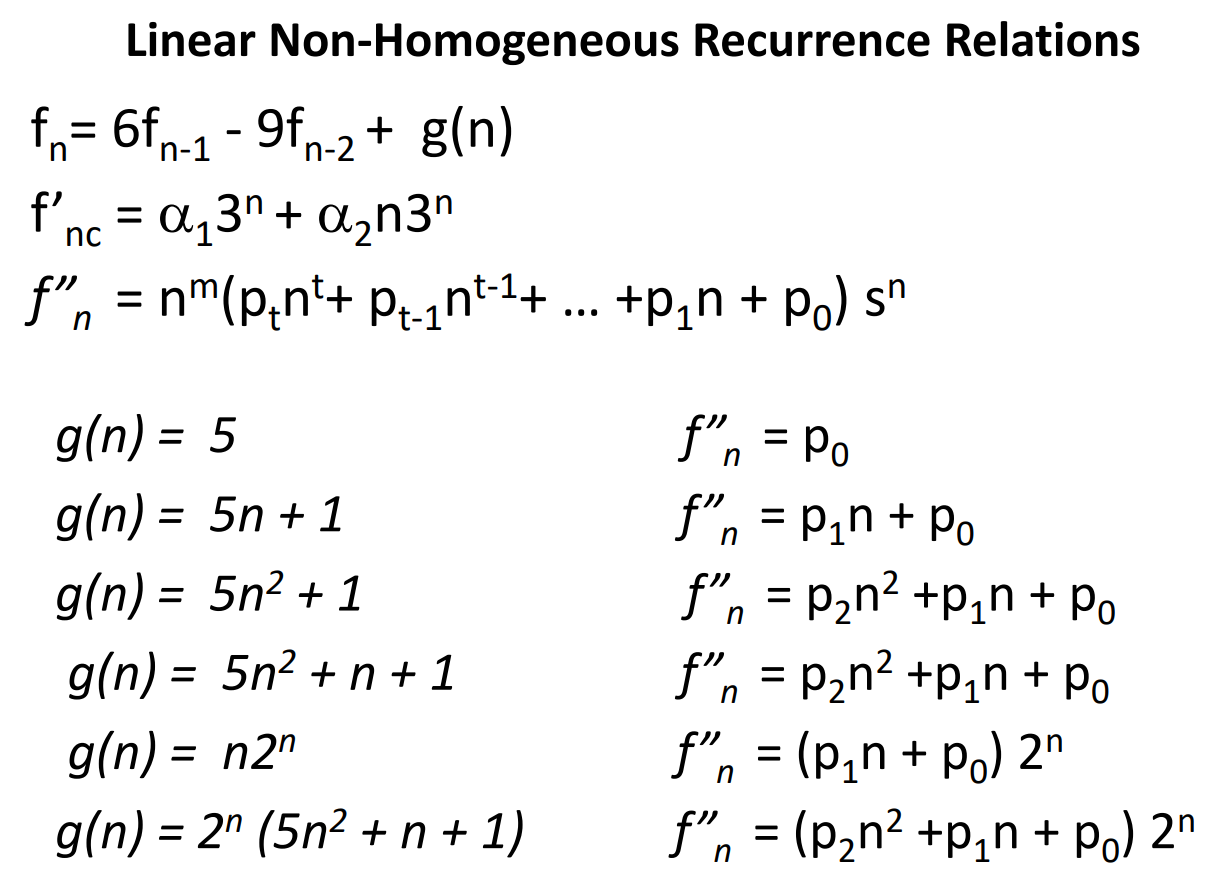
\includegraphics[width=.75\linewidth]{r.png}
\end{frame}

\begin{frame}{Non-homogeneous recurrence}
    \begin{itemize}
        \item Find a particular solution for recurrence relation:
            \begin{equation}\tag{1}
                f_n = 3 \cdot f_{n-1} + f_{n-2} + 6
            \end{equation}
    \end{itemize}
\end{frame}

\begin{frame}{Non-homogeneous recurrence}
    \begin{itemize}
        \item Find a particular solution for recurrence relation:
            \begin{equation}\tag{1}
                f_n = 3 \cdot f_{n-1} + f_{n-2} + 6
            \end{equation}
        \item $g(n) = 6$, so:
            \begin{equation}\tag{2}
                f_n^{''} = p_0
            \end{equation}
    \end{itemize}
\end{frame}

\begin{frame}{Non-homogeneous recurrence}
    \begin{itemize}
        \item Find a particular solution for recurrence relation:
            \begin{equation}\tag{1}
                f_n = 3 \cdot f_{n-1} + f_{n-2} + 6
            \end{equation}
        \item $g(n) = 6$, so:
            \begin{equation}\tag{2}
                f_n^{''} = p_0
            \end{equation}
        \item Plugin $(2)$ in $(1)$ becomes: 
            $$ p_0 = 3 \cdot p_0 + p_0 + 6 $$
            $$ p_0 - p_0 - 3 \cdot p_0 = 6 $$
            \begin{equation}\tag{3}
                p_0 = - \frac{6}{2} =  -2
            \end{equation}
    \end{itemize}
\end{frame}

\begin{frame}{Non-homogeneous recurrence}
    \begin{itemize}
        \item Find a particular solution for recurrence relation:
            \begin{equation}\tag{1}
                f_n = 3 \cdot f_{n-1} + f_{n-2} + 6
            \end{equation}
        \item $g(n) = 6$, so:
            \begin{equation}\tag{2}
                f_n^{''} = p_0
            \end{equation}
        \item Plugin $(2)$ in $(1)$ becomes: 
            $$ p_0 = 3 \cdot p_0 + p_0 + 6 $$
            $$ p_0 - p_0 - 3 \cdot p_0 = 6 $$
            \begin{equation}\tag{3}
                p_0 = - \frac{6}{2} =  -2
            \end{equation}
        \item Finally $(3)$ in $(2)$:
        $$ f_n^{''} = -2 $$
    \end{itemize}
\end{frame}

\begin{frame}{Non-homogeneous recurrence}
   \begin{itemize}
        \item Find a particular solution for recurrence relation:
            \begin{equation}\tag{1}
                f_n = 3 \cdot f_{n-1} + f_{n-2} + 3 \cdot 2^n
            \end{equation}
      \end{itemize}
\end{frame}

\begin{frame}{Non-homogeneous recurrence}
   \begin{itemize}
        \item Find a particular solution for recurrence relation:
            \begin{equation}\tag{1}
                f_n = 3 \cdot f_{n-1} + f_{n-2} + 3 \cdot 2^n
            \end{equation}
        \item $g(n) = 3 \cdot 2^n$:
            \begin{equation}\tag{2}
                f_n^{''} = p_0 \cdot 2^n
            \end{equation}
      \end{itemize}
\end{frame}

\begin{frame}{Non-homogeneous recurrence}
   \begin{itemize}
        \item $(2)$ in $(1)$:
            $$ p_0 \cdot 2^n = 3 \cdot p_0 \cdot 2^{n-1} + p_0 \cdot 2^{n-2} + 3 \cdot 2^n $$
            $$ p_0 \cdot 2^n = 2^{n-2}( 3 \cdot p_0 \cdot 2^{1} + p_0 \cdot 2^{0} + 3 \cdot 2^2) $$
            $$ p_0 \cdot 2^2 = 3 \cdot p_0 \cdot 2 + p_0 + 3 \cdot 4 $$
            $$ p_0 \cdot 4 = 7 \cdot p_0 + 12 $$
            \begin{equation}\tag{3}
                p_0 = -4
            \end{equation}
      \end{itemize}
\end{frame}

\begin{frame}{Non-homogeneous recurrence}
   \begin{itemize}
        \item $(2)$ in $(1)$:
            $$ p_0 \cdot 2^n = 3 \cdot p_0 \cdot 2^{n-1} + p_0 \cdot 2^{n-2} + 3 \cdot 2^n $$
            $$ p_0 \cdot 2^n = 2^{n-2}( 3 \cdot p_0 \cdot 2^{1} + p_0 \cdot 2^{0} + 3 \cdot 2^2) $$
            $$ p_0 \cdot 2^2 = 3 \cdot p_0 \cdot 2 + p_0 + 3 \cdot 4 $$
            $$ p_0 \cdot 4 = 7 \cdot p_0 + 12 $$
            \begin{equation}\tag{3}
                p_0 = -4
            \end{equation}
        \item Finally, $(3)$ in $(2)$:
            $$ f_n^{''} = -4 \cdot 2^n $$
      \end{itemize}
\end{frame}

\begin{frame}{Non-homogeneous recurrence}
    Solve the following non-homogeneous recurrence:
    \begin{equation}\tag{1}
        f_n = 4 \cdot f_{n-1} - 4 \cdot f_{n-2} + 2 \cdot 5^n
    \end{equation}
    with initial condition: $f_0 = 1$ and $f_1 = 2$.
\end{frame}

\begin{frame}{Non-homogeneous recurrence}
    Solve the following non-homogeneous recurrence:
    \begin{equation}\tag{1}
        f_n = 4 \cdot f_{n-1} - 4 \cdot f_{n-2} + 2 \cdot 5^n
    \end{equation}
    with initial condition: $f_0 = 1$ and $f_1 = 2$.
    
    \begin{itemize}
        \item $ f_n^{'} =  4 \cdot f_{n-1} - 4 \cdot f_{n-2}$
        \begin{enumerate}
            \item Caractheristic equations and its roots:
                $$ x^2 - 4 \cdot x + 4 = 0 $$
                $$ (x - 2)(x - 2) = 0 $$
                $$ x_{1,2} = 2 $$
            \item General form of the solution:
                $$ f_n^{'} = \alpha_1 \cdot 2^n + \alpha_2 \cdot n \cdot 2^n $$
        \end{enumerate}
    \end{itemize}
\end{frame}

\begin{frame}{Non-homogeneous recurrence}
    Solve the following non-homogeneous recurrence:
    \begin{equation}\tag{1}
        f_n = 4 \cdot f_{n-1} - 4 \cdot f_{n-2} + 2 \cdot 5^n
    \end{equation}
    with initial condition: $f_0 = 1$ and $f_1 = 2$.
    
    \begin{itemize}
        \item $ g(n) =  2 \cdot 5^n$, so:
            \begin{equation}\tag{2}
                f_n^{''} = p_0 \cdot 5^n
            \end{equation}
        \item $(2)$ in $(1)$:
            $$ p_0 \cdot 5^n = 4 \cdot p_0 \cdot 5^{n-1} - 4 \cdot p_0 \cdot 5^{n-2} + 2 \cdot 5^n $$
            \begin{equation}\tag{3}
                p_0 = 2
            \end{equation}
        \item Finally, $(3)$ in $(2)$:
            $$ f_n^{''} = 2 \cdot 5^n $$
    \end{itemize}

    %\\$A_{0}=\alpha_1+2=1$
    %\\$A_{1}=2\alpha_1+2\alpha_2+10=2$
    %\\$\alpha_1=-1 ,\alpha_2=-3$
\end{frame}

\begin{frame}{Non-homogeneous recurrence}
    Solve the following non-homogeneous recurrence:
    \begin{equation}\tag{1}
        f_n = 4 \cdot f_{n-1} - 4 \cdot f_{n-2} + 2 \cdot 5^n
    \end{equation}
    with initial condition: $f_0 = 1$ and $f_1 = 2$.
    
    \begin{itemize}
        \item $ f_n^{'} = \alpha_1 \cdot 2^n + \alpha_2 \cdot n \cdot 2^n $
        \item $ f_n^{''} = 2 \cdot 5^n $
        \begin{enumerate}[3]
            \item Initial condition equations and their solutions:
                $$ f_0 = \alpha_1 \cdot 2^0 + \alpha_2 \cdot 0 \cdot 2^0 + 2 \cdot 5^0  = \alpha_1 + 2 = 1 $$
                $$ f_1 = \alpha_1 \cdot 2^1 + \alpha_2 \cdot 1 \cdot 2^1 + 2 \cdot 5^1  = 2 \cdot \alpha_1 + 2 \cdot \alpha_2 + 10 = 2 $$
                $$ \alpha_1 = -1 $$
                $$ \alpha_2 = -3 $$
            \item[4] Final answer:
                $$ \vdots $$
        \end{enumerate}
    \end{itemize}
\end{frame}

\section{Divide and Conquer}

\begin{frame}{Divide and Conquer}
    \centering
    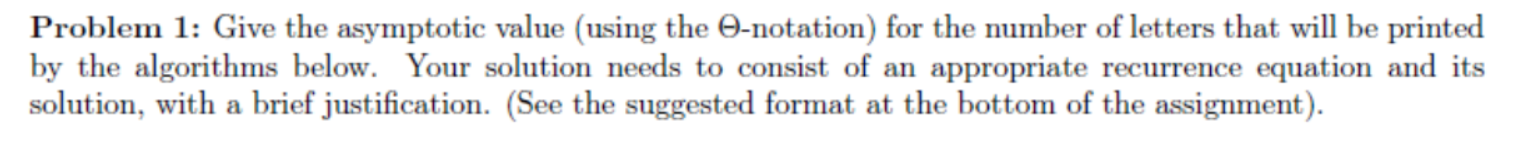
\includegraphics[width=.85\linewidth]{a.PNG}
\end{frame}
\begin{frame}{Divide and Conquer}
    \centering
    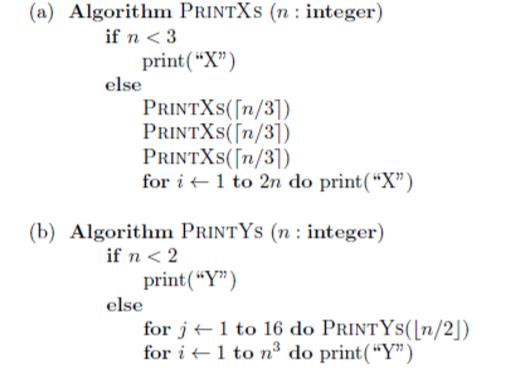
\includegraphics[width=.5\linewidth]{a0.PNG}
\end{frame}
\begin{frame}{Divide and Conquer}
    \centering
    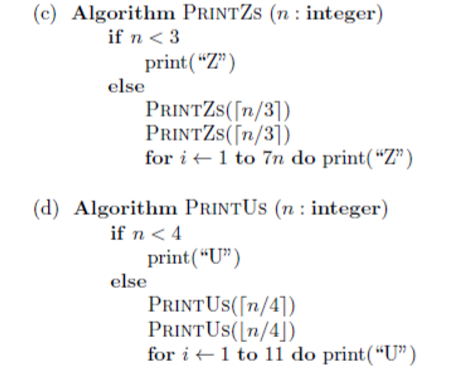
\includegraphics[width=.5\linewidth]{a1.PNG}
\end{frame}
\begin{frame}{Divide and Conquer}
    \centering
    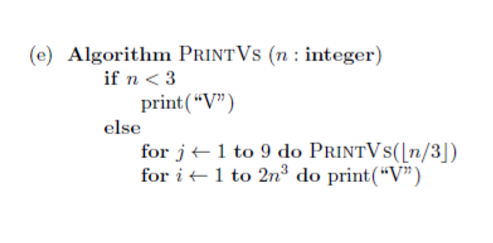
\includegraphics[width=.5\linewidth]{a2.PNG}
\end{frame}
\begin{frame}{Divide and Conquer}
    \centering
    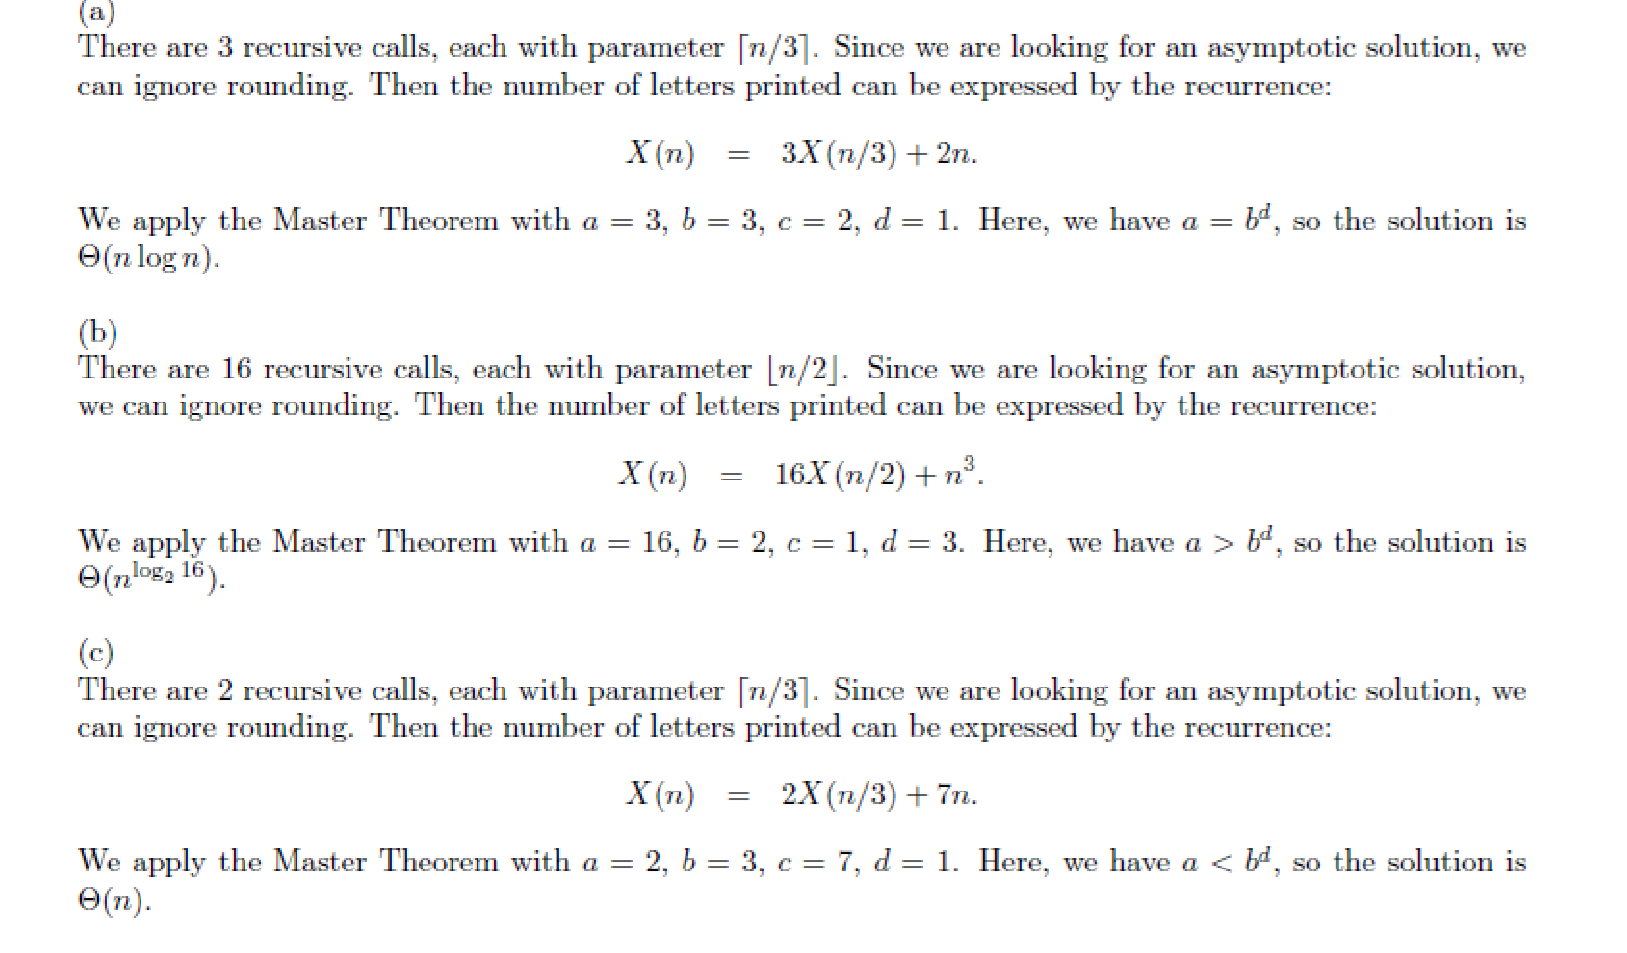
\includegraphics[width=.95\linewidth]{c.PNG}
\end{frame}
\begin{frame}{Divide and Conquer}
    \centering
    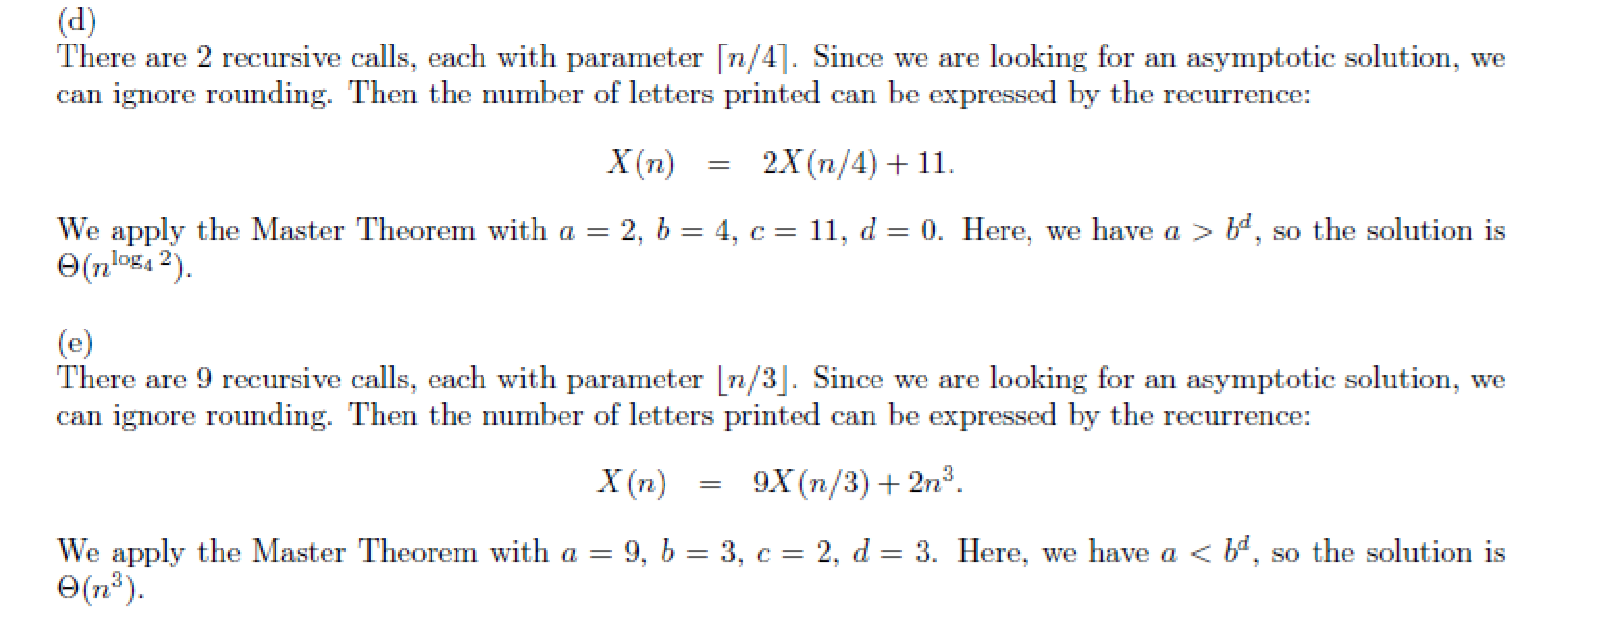
\includegraphics[width=.95\linewidth]{e.PNG}
\end{frame}

\section{Inclusion-Exclusion }

\begin{frame}{Inclusion-Exclusion}
    \centering
    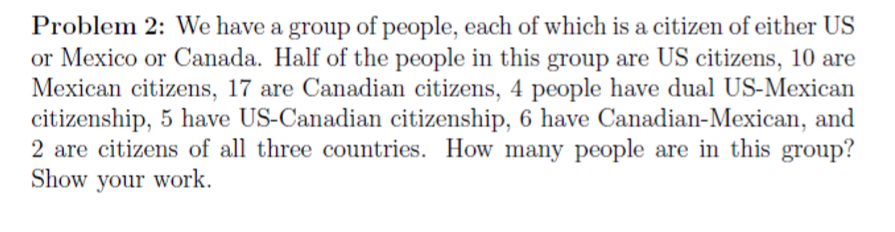
\includegraphics[width=.7\linewidth]{3.PNG}
\end{frame}
\begin{frame}{Inclusion-Exclusion}
    \centering
    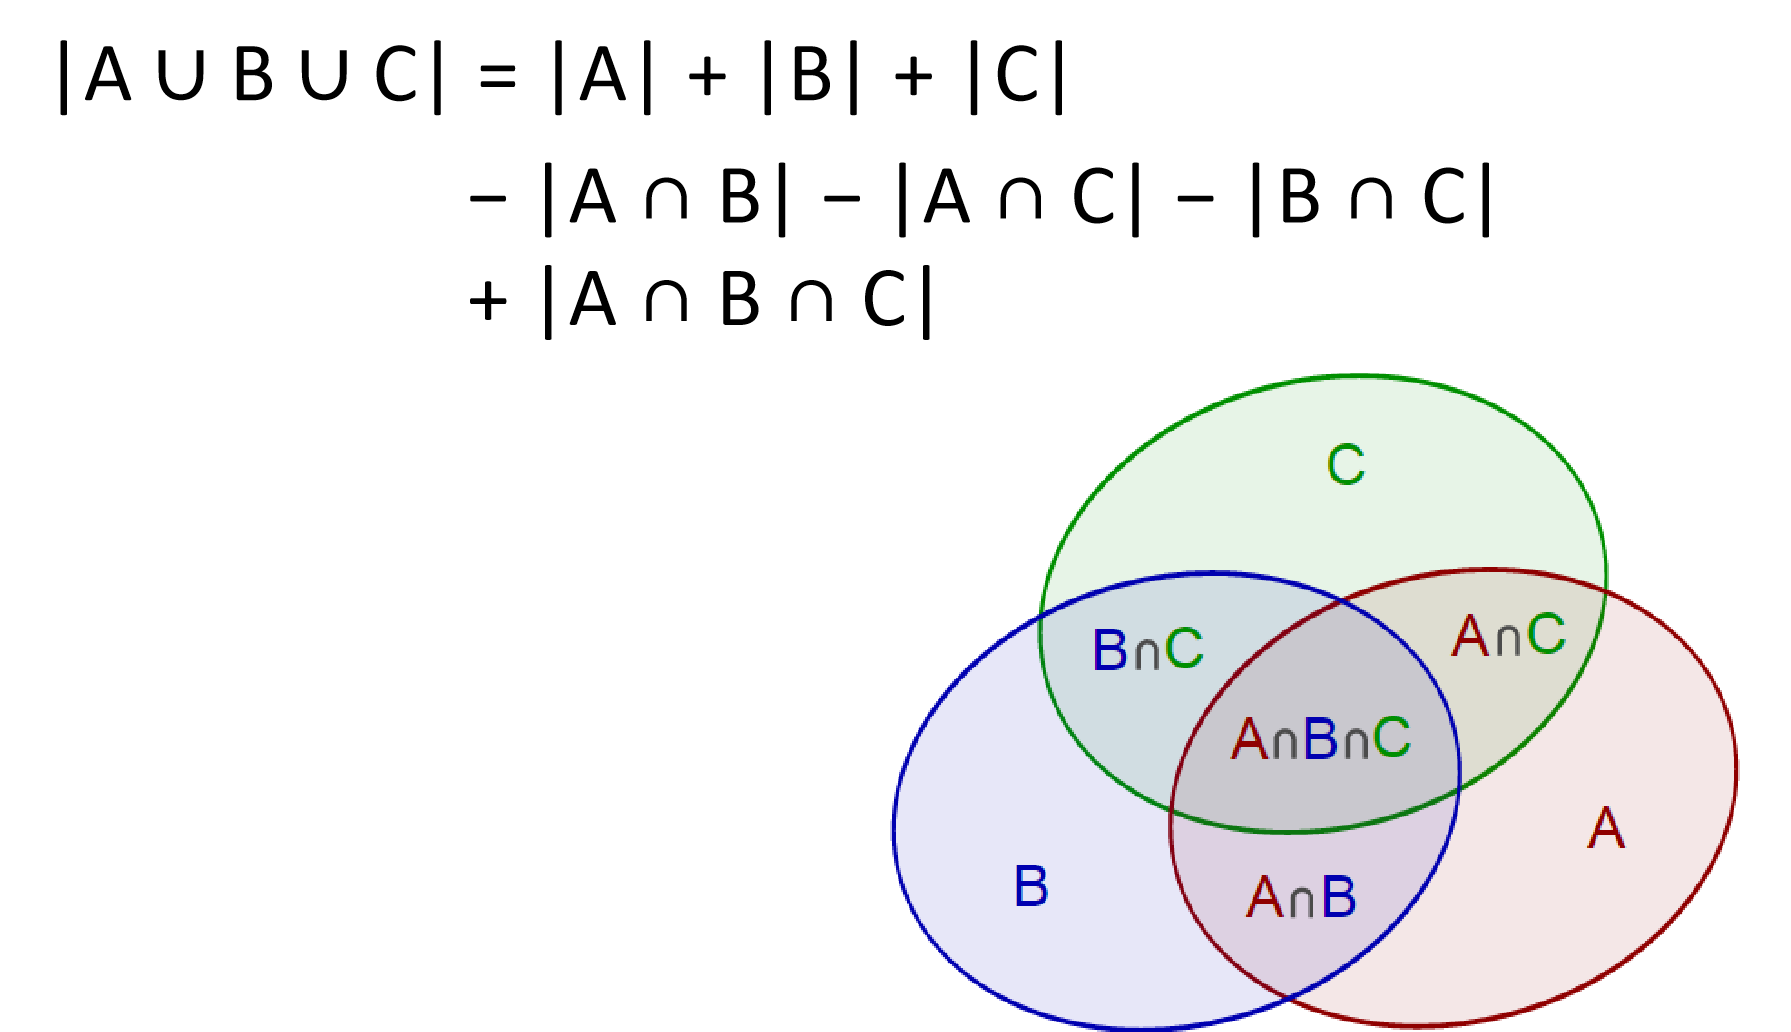
\includegraphics[width=.7\linewidth]{4.PNG}
\end{frame}

\begin{frame}{Inclusion-Exclusion}
    \centering
    \begin{tabular}{r c l}
    Us citizens:                & $\mid A \mid$                & $= \frac{X}{2}$    \\
    Mexican citizen:            & $\mid B \mid$                & $= 10$             \\
    Canadian citizen:           & $\mid C \mid$                & $= 17$             \\
    US-Mexican citizen:         & $\mid A \cap B \mid$         & $= 4$              \\
    US-Canadian citizen:        & $\mid A \cap C \mid$         & $= 5$              \\
    Canadian-Mexican:           & $\mid B \cap C \mid$         & $= 6$              \\
    Citizens of all countries:  & $\mid A \cap B \cap C \mid$  & $= 2$              \\
    \end{tabular}

    $$X = \frac{X}{2} + 10 + 17 - 4 - 5 - 6 + 2$$
    $$X = \frac{X}{2} + 14$$
    $$X = 28$$

\end{frame}


\end{document}
